\documentclass[10pt,a4paper]{article}
\usepackage[margin=2.1cm]{geometry}
\usepackage[T1]{fontenc}
\usepackage{lmodern}
\usepackage{microtype}
\usepackage{graphicx}
\usepackage{booktabs}
\usepackage{tabularx}
\usepackage{longtable}
\usepackage{array}
\usepackage[table]{xcolor}
\usepackage{enumitem}
\PassOptionsToPackage{obeyspaces,spaces}{url}
\usepackage{hyperref}
\def\UrlBreaks{\do\/\do\_\do\-\do\.\do\<\do\>}
\usepackage{fancyhdr}
\usepackage{titlesec}
\usepackage{needspace}

\definecolor{accent}{HTML}{1D4E9E}
\definecolor{soft}{HTML}{EEF3FB}
\hypersetup{colorlinks=true, linkcolor=accent, urlcolor=accent}
\titleformat{\section}{\large\bfseries\color{accent}}{\thesection}{0.6em}{}
\titleformat{\subsection}{\normalsize\bfseries}{\thesubsection}{0.5em}{}
\setlist{nosep, leftmargin=1.4em}
\setlength{\parskip}{0.45em}
\setlength{\parindent}{0pt}
\renewcommand{\arraystretch}{1.25}
\newcolumntype{L}{>{\raggedright\arraybackslash}X}
\newcommand{\file}[1]{\nolinkurl{#1}}
\newcommand{\keybox}[1]{\par\noindent\colorbox{soft}{\parbox{\dimexpr\linewidth-2\fboxsep}{#1}}\par}

\pagestyle{fancy}
\fancyhf{}
\lhead{\small Flame in Freefall --- team status}
\rhead{\small 14 Nov 2026}
\cfoot{\small \thepage}

\begin{document}

\begin{center}
{\LARGE\bfseries Flame in Freefall}\\[0.3em]
{\large Team status, data review and plan to submission}\\[0.4em]
{\small NASA Space Apps 2026 \textbullet{} prepared by Mahmoud Nadeem with AI assistance (Claude) \textbullet{} Saturday 14 Nov 2026, 19:15 Cairo}
\end{center}

\keybox{\textbf{In one paragraph.} The challenge asks for an SI-powered dashboard that \emph{summarises, ranks and interprets} PSI combustion investigations for crew habitats. The leader's mission-advisor idea (``I am going to the Moon with this vehicle --- what do I need to know?'') fits that ask, and the work done today supplies its engine: a verified inventory of all 24 combustion investigations, the files in each that hold processed results or telemetry, and an oxygen-versus-pressure analysis of 1,009 tests. Its headline: only 20 tests burned with Moon-base-level oxygen in the chamber atmosphere, all gas flames, and no solid material was ever tested above 22.2\% O$_2$. The catalog was then pulled live for all 24 investigations and the headline numbers reproduce exactly on the downloaded tables. The assignment sheet checks out: every DOI matches the PSI API, the three unknown IDs are found, and four small ground studies are still unassigned.}


\section{The challenge, the rules and how we are judged}

\textbf{Ask.} Build an SI-powered, web-based dashboard that summarises, ranks and interprets combustion science investigations in NASA's Physical Sciences Informatics (PSI) repository to give fire-safety insight for spacecraft, space stations, lunar and Martian bases and pressurized rovers. Suggested user abilities: (1) identify the investigations most relevant to each habitat, (2) extract data that supports predictive modeling of flammability and fire scenarios, (3) highlight research that informs next-generation fire-safety controls and equipment; optionally, Earth applications.

\textbf{Hints the judges wrote into the statement} (each one we visibly answer is cheap credit): show objectives, fuels with sample or burner shape and size, oxygen and air-flow conditions, what varied and what stayed the same between tests, sensors; compare investigations; DAFT used a SAME instrument to measure dust; ACME BRE studied material flammability with gas burners; the three hardware families (ACME in the CIR, MDCA in the CIR, MSG with the SPICE flow duct); spacesuits run 100\% O$_2$ at 4.3\,psi, a Moon base likely $\geq$30\% O$_2$ at $\leq$10.2\,psi; CFI-G reached 85\% O$_2$; PSI holds no partial-gravity data, E-FIELD mimics it, and microgravity and normal-gravity results bound it.

\textbf{Out of scope.} Rocket and propellant fires (footnote of the statement). Questions about ``the fuel the vehicle uses'' should be read as cabin materials, liquid spills and gas leaks.

\begin{tabularx}{\linewidth}{@{}lL@{}}
\toprule
\textbf{Rule (Submission Guide)} & \textbf{What it means for us}\\
\midrule
Judging criteria & Impact, Creativity, Validity, Relevance, Presentation.\\
Demo & A video of 30\,s or less, \emph{or} at most 7 slides; publicly accessible link, no login.\\
Language & English everywhere; Arabic speech only with English subtitles.\\
SI use & Allowed and must be disclosed; AI images need a visible watermark; SI must not be used to come up with the idea of how to solve the challenge. The team's own concept stays the base.\\
Branding & No NASA logos, flags or mission identifiers in generated content.\\
NASA data & At least one NASA data source is required for global awards (we use PSI throughout).\\
Deadline & Sunday 15 Nov, 23:59 local time; we aim to submit at 22:00.\\
\bottomrule
\end{tabularx}

\section{The leader's vision, and what the data can really answer}

The leader's flow: a user (researcher, engineer) states a mission (e.g.\ lunar surface, spacecraft or rover), the system asks follow-up questions (materials, liquids or gases on board, goal: prevention, detection or suppression), then shows oxygen effects, flammability, burning rates, ignition, detection and prevention guidance, with a chatbot on top. This matches the challenge's first ask almost word for word. To keep Validity high, every answer must state what PSI measured, under which conditions, and where the data stops.

\begin{tabularx}{\linewidth}{@{}p{4.1cm}p{2.1cm}L@{}}
\toprule
\textbf{Question in the advisor flow} & \textbf{PSI can answer?} & \textbf{Where, and the limit}\\
\midrule
Which materials should I use? & Partly & What burned, how fast, at what O$_2$ and flow: BASS, BASS-II, SAFFIRE I--III, BRE (gas emulator). No solid tested above 22.2\% O$_2$, so no evidence-based ranking at Moon O$_2$. Phrase as evidence, never as a recommendation.\\
How does oxygen change the fire? & Yes & O$_2$ sweeps: CFI-G (12--85\%), Flame Design (20--85\%), FLEX (12--34\%), BRE (21--40\%), BASS-II (13.6--22.2\%).\\
More or less flammable than on Earth? & Partly & Microgravity vs 1-g columns in SAFFIRE-II, BASS's link to NASA-STD-6001, SPICE ground tests. Lunar gravity: no data; bounded by $\mu g$ and 1-g, with E-FIELD as a proxy.\\
Evaporation / burning rate & Yes, liquids & FLEX burning-rate constant $k$ (0.05--1.06\,mm$^2$/s) and 30\,fps droplet diameters for 258 tests.\\
Ignition temperature & No, indirectly & No ignition temperature is measured; CFI-G gives hot-ignition yes/no, peak burner temperature and adiabatic flame temperature; cool flames burn at about 500--1,000\,K.\\
What starts fires? & Partly & SAME heated real cabin materials (Kapton wire insulation, silicone, Teflon) until they smoked: overheating before flame.\\
Detection & Yes & SAME and SAME-R: ISS and Shuttle detectors, ionization detectors, particle counter and photometers, particle size; DAFT: same instrument types on dust.\\
Suppression & Yes & FLEX: CO$_2$ and helium dilution, 274 labeled outcomes.\\
Fuel of the vehicle & Out of scope & Propellants are excluded; treat as cabin liquids and gas leaks.\\
\bottomrule
\end{tabularx}

\section{What was done today}

\begin{enumerate}
\item \textbf{Morning, before the challenge text arrived:} studied the PSI repository (26 search hits for ``combustion''), reverse-engineered its public JSON API, read real files of 6 investigations and wrote a dataset study (living doc linked at the end).
\item \textbf{Midday, after the challenge text:} corrected the plan (the product is a dashboard over all investigations; models are one module), corrected two Flame Design facts, and designed the platform and contribution format.
\item \textbf{Inventory:} metadata, file trees and experimental tables of all 24 combustion investigations through the API (sizes, file types, which files are processed results or telemetry).
\item \textbf{Analysis:} oxygen and pressure of every test in six experimental tables against the habitat envelopes in the statement (Section~\ref{sec:finding}).
\item \textbf{Code:} a tested Python pipeline and contribution repo in \file{Project 3-nasa/flame-in-freefall} (Section~\ref{sec:built}).
\item \textbf{Evening:} checked the assignment sheet line by line against the API; result in \file{psi_member_assignments_verified.csv} (Section~\ref{sec:review}).
\item \textbf{Evening, live run:} the catalog builder ran on Mahmoud's laptop and downloaded the metadata of all 24 investigations and their 22 experimental tables; the full pipeline on those files reproduces the headline exactly (1,009 tests; 20 ambient and 46 burner-oxygen tests inside the envelope; 17 FLEX tests just outside).
\end{enumerate}

\section{Review of the assignment sheet}\label{sec:review}

\textbf{Verdict: the split is good and every DOI is right.} All 20 rows were checked against the PSI API on 14 Nov. Corrections and additions:

\begin{itemize}
\item \textbf{IDs found:} FLEX-2 is \textbf{PSI-68}, E-FIELD Flames is \textbf{PSI-22}, s-Flame is \textbf{PSI-23}. PSI-26 is confirmed as BASS (DOI 10.60555/58h4-dy80). The ``third-party'' DOIs all match PSI.
\item \textbf{SPICE size:} 6.95\,GB in decimal units is 6.47\,GiB; the pasted ``6.47\,GB'' is the same size in binary units.
\item \textbf{DAFT:} one record (PSI-47) covers both DAFT and DAFT-2.
\item \textbf{Unassigned ground studies:} PSI-62 (flame-spread modeling vs BASS, metadata only) $\rightarrow$ T1; PSI-115 (SAME smoke CFD, 44 output files) $\rightarrow$ T3; PSI-117 (cool-flame CFD with FLEX) and PSI-142 (counterflow cool flames) $\rightarrow$ T4.
\item \textbf{Workload balance:} T4 (Tamer) and T5 (Adawi) each hold about 2\,TB investigations, but only their small processed files are needed (table below); T2 (Shreif) holds only 13 SAFFIRE samples in total, so his strength is visuals and the spacecraft-scale story, not model training.
\end{itemize}

\begin{longtable}{@{}p{2.3cm}p{2.6cm}p{1.6cm}p{6.1cm}p{1.6cm}@{}}
\toprule
\textbf{Member} & \textbf{Investigation} & \textbf{ID} & \textbf{Processed results / telemetry to use first} & \textbf{Priority}\\
\midrule
\endhead
Amr Morgan & BASS & PSI-26 & 114 flight videos; table has material only (no O$_2$) & Medium\\
 & BASS-II & PSI-25 & Table with O$_2$, CO$_2$, CO before and after (129 tests); 296 videos & High\\
Mohamed Shreif & SAFFIRE-I, II, III & PSI-98, 99, 100 & Raw-data workbooks (4 / 11 / 6 \file{.xlsx}); 2 + 9 + 2 samples & Medium\\
Mahmoud Nadeem & SAME & PSI-102 & 59 analyzed \file{.xls}; per-test results in the SAME-R workbook & High\\
 & SAME-R & PSI-101 & \file{SAME, SAME-R_Results.xlsx} (154 tests) + 44 detector logs at 1\,Hz & High\\
 & DAFT / DAFT-2 & PSI-47 & 6 time series (P-Trak, DustTrak) + 12 analyzed \file{.xls} & Med.--High\\
Mohammed Tamer & FLEX & PSI-69 & 258 tests: droplet and flame size at 30\,fps (\file{.txt}, about 20\,MB) & High\\
 & FLEX-2 & PSI-68 & Per-test telemetry \file{.txt} (0.53\,GB); no extracted diameters & Medium\\
 & CFI & PSI-39 & Radiometer and chamber readings per test (about 170\,MB) & Medium\\
 & CFI-G & PSI-159 & 338 sensor logs \file{*_data.csv} (36 channels, 1.46\,GB); 333 labeled tests & High\\
Khaled Adawi & BRE & PSI-20 & 187 sensor logs (1.09\,GB); 194 flames at 21--40\% O$_2$ & High\\
 & E-FIELD & PSI-22 & 204 sensor logs (1.52\,GB); partial-gravity proxy & Med.--High\\
 & s-Flame & PSI-23 & 288 sensor logs (0.77\,GB); some days at about 30\% O$_2$ & Medium\\
 & Flame Design & PSI-10 & 317 sensor logs (1.25\,GB); 327 tests & High\\
Mohamed Gamal & SPICE & PSI-107 & Flame-length and flight-data workbooks; 469 flames & Medium\\
 & SLICE & PSI-106 & No results table: 22,990 raw image frames & Low\\
 & CLD Flame & PSI-21 & 404 sensor logs (1.38\,GB) & Medium\\
\bottomrule
\end{longtable}

The full table, with sizes, file counts, experimental-table rows and per-investigation quirks, is \file{psi_member_assignments_verified.csv} in the Project 3-nasa folder. The leader's original file is untouched.

\section{Headline finding: the Moon-base oxygen gap}\label{sec:finding}

\begin{center}
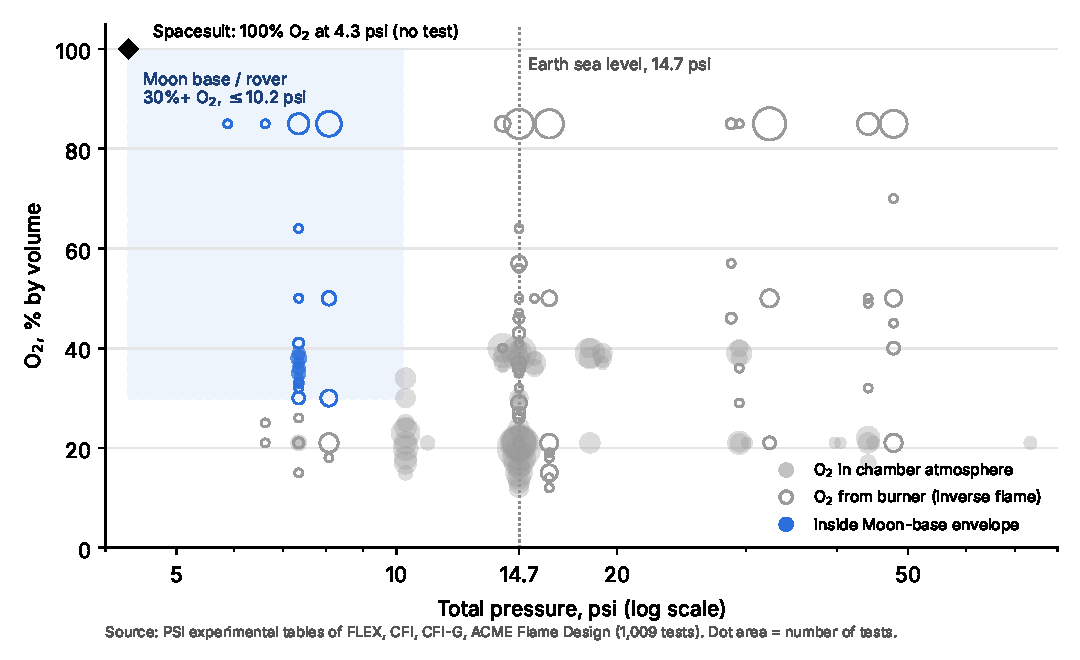
\includegraphics[width=0.92\linewidth]{envelope.pdf}
\end{center}

\textbf{Method.} Six experimental tables record oxygen and pressure per test: FLEX, CFI, CFI-G (normal and inverse) and ACME Flame Design (normal and inverse); 1,021 tests, 1,009 with both values. Each test is compared with the envelopes in the statement.

\begin{tabularx}{\linewidth}{@{}lL@{}}
\toprule
\textbf{Group} & \textbf{Tests inside the Moon-base envelope ($\geq$30\% O$_2$, 4.3--10.2\,psi)}\\
\midrule
CFI-G normal flames (O$_2$ in the atmosphere) & 20 (17 ignited a hot flame, 3 did not)\\
CFI-G and Flame Design inverse flames (O$_2$ from the burner) & 28 + 18 = 46\\
FLEX droplets & 0; 17 just outside at 30--34\% O$_2$ and 10.3--10.5\,psi (14 disrupted, 3 burned out, none extinguished)\\
Solid materials & 0: BASS-II never exceeded 22.2\% O$_2$; SAFFIRE ran near 21.5--22.1\%\\
Spacesuit atmosphere & 0: the lowest pressure of any test is 0.42\,atm (6.2\,psi)\\
\bottomrule
\end{tabularx}

\textbf{Meaning.} Fabrics and plastics are what burn in a habitat, yet PSI's microgravity data at Moon-base oxygen levels are gas flames and a gas-fed emulator (BRE, 21--40\% O$_2$, pressure not tabulated). Any prediction of solid-material flammability for a Moon base extrapolates; solid tests at $\geq$30\% O$_2$ and about 10\,psi are the largest open gap. \textbf{Caveats:} values come from experimental tables only; RAMP and LOW O$_2$ entries and FLEX test 114 (pressure 0) are excluded.

\section{Strong opportunities to add}

\begin{tabularx}{\linewidth}{@{}p{3.3cm}p{3.3cm}L@{}}
\toprule
\textbf{Opportunity} & \textbf{Data} & \textbf{Why it scores, and the risk}\\
\midrule
Dust vs smoke false alarms on the Moon & DAFT (PSI-47) + SAME / SAME-R & The statement hints at it. Lunar dust can trip smoke detectors; the same instrument types measured both. Particle count vs mass separates fine smoke from coarser dust. Risk: DAFT is small and its two instruments ran in different sessions, so present as a finding with a physical argument, not a trained model.\\
Habitat advisor + gap map & All experimental tables & Already computed; it is the engine of the leader's flow and the strongest 5 seconds of the video.\\
Suppressant effectiveness & FLEX & CO$_2$ vs helium vs nitrogen dilution with 274 labeled outcomes: classifier and an oxygen--diluent map. Baseline to beat: 68\% (always ``extinction'').\\
Oxygen sensitivity curves & BRE, CFI-G & Ignition and self-extinction vs O$_2$ and pressure: the core of ``what changes on the Moon''.\\
Partial-gravity bound & E-FIELD + $\mu g$ vs 1-g pairs & The statement names it; one honest panel that says what can and cannot be bounded.\\
Detector telemetry & SAME-R 1\,Hz logs & Which detector alarms first for each material: directly ``next-generation detection equipment''.\\
\bottomrule
\end{tabularx}

\section{Platform decisions}

\textbf{Architecture.} Members add files; a Python pipeline checks them, merges them with PSI data and builds everything the site and the chatbot read. Adding the 25th dataset needs no code change.

\begin{tabularx}{\linewidth}{@{}p{3.2cm}p{4.4cm}L@{}}
\toprule
\textbf{Topic} & \textbf{Decision} & \textbf{Reason}\\
\midrule
Warehouse & One SQLite file built by the pipeline: tables for investigations, cards, findings, models, members, tests, files, plus text chunks for retrieval & Tables and text in one place, as the leader asked; Python's standard library reads it; one file to version and ship. Status: to build (about 1 hour).\\
SI text & Hosted LLM API, called by the pipeline; outputs cached and labeled as SI-generated & Numbers come only from data; the SI writes the words around them.\\
Chatbot & Retrieval over the text chunks + hosted LLM behind one small serverless function holding the key; answers must cite PSI IDs & A judge's browser cannot run a local model, and the key must never be in the repo.\\
Local model & Only as an offline fallback & \emph{Coqui} is a text-to-speech library, not a text-analysis model; if a local model was meant, an open LLM such as \emph{Qwen} fits.\\
Judged link & Must never sleep & Streamlit Community Cloud apps sleep after 12\,h without traffic (Streamlit docs); a static site on GitHub Pages does not. If Streamlit is chosen for speed, add a static snapshot and the video.\\
\bottomrule
\end{tabularx}

\section{How each member hands over work}

The leader asked for one fixed handover format. Proposal, already built: every contribution is a file in \file{content/}, and it counts as handed over when \file{python -m pipeline.validate} prints \texttt{OK}. Each item shows on the site under its author's name.

\begin{tabularx}{\linewidth}{@{}p{2.6cm}p{4.6cm}L@{}}
\toprule
\textbf{You add} & \textbf{Where} & \textbf{Must contain}\\
\midrule
Investigation card & \file{content/investigations/<PSI-ID>/card.yaml} & Summary, fuels, sample shape and size, O$_2$ / pressure / flow ranges, what varied, what stayed the same, sensors, pillars, data readiness, sources\\
Finding & \file{content/findings/<slug>.md} & A claim with a number, evidence (path, URL or DOI), confidence, SI disclosure\\
Mini-model & \file{content/models/<id>/model.yaml} & Target, inputs, validation method, metrics \emph{and} a baseline, limitations\\
\bottomrule
\end{tabularx}

Templates are in \file{templates/}, instructions in \file{CONTRIBUTING.md}. Members who do not use Git send the filled files to the integrator.

\textbf{Attribution, done.} This morning, before the sheet existed, Mahmoud drafted cards for FLEX, CFI-G, Flame Design, BRE and BASS-II, which belong to other tracks. Each card now carries its track owner as author, with a two-line note at the top: the owner verifies every field against the PSI page, completes it and deletes the note. Mahmoud keeps SAME-R (his track) and the cross-investigation finding.

\section{Built and verified}\label{sec:built}

\begin{tabularx}{\linewidth}{@{}p{3.6cm}L p{3.6cm}@{}}
\toprule
\textbf{Part} & \textbf{Verified} & \textbf{Not yet verified}\\
\midrule
PSI API client & All four endpoints in a browser session, then a live Python run on Mahmoud's laptop & ---\\
Catalog builder & Live run: 24 investigations, 22 experimental tables; drops contact e-mails & ---\\
Browser fallback & Export run on real data; import tested on a real record & Not needed so far\\
Envelope + ranking & Re-run on the downloaded tables reproduces every headline number & Ranking weights are judgment\\
Validator + schemas & Tests including a deliberately broken card & ---\\
Site export & End-to-end run writes \file{site_data/*.json} for 24 investigations & Front end not started\\
Whole repo & 24 tests pass in the build environment and in a clean Python 3.10 environment on Mahmoud's computer & ---\\
\bottomrule
\end{tabularx}

\section{What to send to the team now, and the plan}

\textbf{Send tonight}\par
\begin{enumerate}
\item To the leader: this PDF, \file{psi_member_assignments_verified.csv} (IDs found, DOIs confirmed, 4 unassigned studies, files to use per investigation) and \file{flame-in-freefall_2026-11-14.zip} (the repo, with all 24 investigations already pulled).
\item To everyone: the column ``Processed or telemetry files to use first'' for their own rows, so nobody downloads terabytes of images.
\item To everyone: the handover format (Section 8) with \file{CONTRIBUTING.md} and \file{templates/}.
\item To the group: \file{envelope.png}, the headline finding as one picture.
\item To the call: the decisions in Section 7, the out-of-scope note on propellants, and the attribution change.
\end{enumerate}

\needspace{12\baselineskip}
\textbf{Plan to submission (Cairo time)}\par\smallskip
\begin{tabularx}{\linewidth}{@{}p{3.2cm}L@{}}
\toprule
\textbf{When} & \textbf{Done when}\\
\midrule
Sat, by 23:00 & Every member has studied their investigations and handed over cards and at least one finding (catalog for all 24 investigations: done).\\
Sun, by 12:00 & Warehouse file and site data built from all contributions; front end shows catalog, investigation pages and the gap map.\\
Sun, by 16:00 & Advisor flow, ranking, chatbot with citations, mini-models with baselines.\\
Sun, by 19:00 & Public link tested in a private window; offline copy ready.\\
Sun, by 21:00 & 30-second video with English subtitles; project page text with NASA data and SI disclosure.\\
Sun, 22:00 & Submit.\\
\bottomrule
\end{tabularx}

\appendix
\section{Data quirks every member should know}
\begin{itemize}
\item Read numbers strictly: ``RAMP'', ``LOW O2'', ``$\sim$21.5'' are not numbers (one script read ``LOW O2'' as 2.0).
\item FLEX: test 114 pressure is 0 (missing); column ``CO'' is CO$_2$; ``Burning rate; mm'' is $k$ in mm$^2$/s; \file{.txt} files use old Mac line endings.
\item ACME \file{*_data.csv}: line 1 is metadata, the header is line 2; time is \texttt{HH:MM:SS:mmm}; channels look like raw volts.
\item CFI-G labels mix ``Yes'', ``yes'', ``flash'' and ``-''; Flame Design has 60 ramped normal tests and 11 inverse tests without an O$_2$ value.
\item SAME workbook: 43 sheets, header on row 2; detector logs use $-999$ for missing.
\item BRE: O$_2$ is a list per day; two cells read ``3400\%'' and ``2100\%''.
\item Some listed files are missing in storage (S3 ``NoSuchKey''); record them, do not stop.
\item Sizes: PSI's ``GB'' may be binary (GiB); 6.95\,GB = 6.47\,GiB.
\end{itemize}

\section{Links and commands}
\begin{itemize}
\item Platform design and contribution guide: \url{https://claude.ai/artifact/VtWu2b9QWiG86PWryKQp9N}
\item Day-1 dataset study: \url{https://claude.ai/artifact/QujwcSKje45vY5SPcsUnkf}
\item PSI combustion search: \url{https://psi.nasa.gov/physci/repo/search?q=combustion}
\end{itemize}
\begin{verbatim}
pip install -r requirements.txt
python -m pipeline.build_catalog     # PSI metadata + experimental tables (needs internet)
python -m pipeline.validate          # check contributions
python -m pipeline.build             # validate, envelope, rank, export site data
python scripts/psi_fetch.py --list-only
\end{verbatim}

\end{document}
